\documentclass[twocolumn,10pt,a4paper]{article}

\usepackage[margin=1.9cm,columnsep=0.85cm]{geometry}
\linespread{1.06}
\setlength{\parskip}{0.4em}
\setlength{\parindent}{0pt}
\setlength{\emergencystretch}{3em}
\hyphenpenalty=1200
\usepackage{enumitem}
\setlist[itemize]{leftmargin=1.1em,itemsep=1pt,topsep=2pt,parsep=0pt}
\usepackage{amsmath,amssymb}
\usepackage{booktabs}
\usepackage{tikz}
\usepackage{xcolor}
\usepackage{microtype}
\usepackage{multicol}
\usepackage[colorlinks=true,linkcolor=blue!55!black,citecolor=blue!55!black,
            urlcolor=blue!55!black]{hyperref}
\usetikzlibrary{positioning,fit,calc}

% pgfplots is not installed in this TeX tree, so every chart below is drawn with
% base TikZ: manual axes plus \draw plot coordinates.
\definecolor{cstruct}{RGB}{20,90,170}
\definecolor{clex}{RGB}{190,80,20}
\definecolor{cbad}{RGB}{170,30,40}
\definecolor{cgood}{RGB}{25,120,60}
\definecolor{cgrey}{RGB}{120,120,120}

\newcommand{\code}[1]{\texttt{\small #1}}

% Axis frame helper: #1 xmin #2 xmax #3 ymin #4 ymax
\newcommand{\axesframe}[4]{%
  \draw[cgrey,very thin] (#1,#3) rectangle (#2,#4);
}

\title{\vspace{-1.2em}\bfseries Meaning-preserving text simplification\\
by activation steering}
\author{Technical report}
\date{30 July 2026}

\begin{document}
\maketitle

\begin{abstract}
\noindent
We steer a 3B instruction-tuned language model toward simpler text by adding a
fixed direction to its residual stream during generation. Two candidate axes are
tested: sentence structure and word difficulty. The axes are separable
directions, mean absolute cosine $0.223$, and they respond at different depths:
structure at layers 15 to 17 of 28, vocabulary at layers 19 to 26. Structural
steering at layer 15 with strength $0.75$ beats prompt-only simplification on
ASSET by SARI $+5.47$ (95\% CI $+2.45$ to $+8.49$) and by bidirectional-NLI
faithfulness $+0.36$ (CI $+0.23$ to $+0.50$), both significant at $n{=}32$.
Against no intervention it is a SARI tie ($+0.43$, CI $-1.75$ to $+2.61$) with
faithfulness unchanged, while cutting sentence length 18\% at zero degeneration.
Prompt-only simplification is significantly worse than no intervention
($-5.04$ SARI): it reaches a low readability grade by deleting and inventing
content. The lexical axis does not pay for itself, so the deliverable is one
dial. We also report a floating-point defect on Apple MPS that silently
corrupted every extracted vector and produced a false negative result, and two
metric defects that inverted conclusions.
\end{abstract}


\begin{figure}[!t]
\centering
\fbox{\parbox{0.93\columnwidth}{\small
\textbf{Result.} One dial, structural, layer 15, $\alpha=0.75$.\\[0.3em]
\begin{tabular}{@{}lr@{}}
vs.\ prompt-only, SARI      & $+5.47$ \; [$+2.45$, $+8.49$] \\
vs.\ prompt-only, NLI       & $+0.36$ \; [$+0.23$, $+0.50$] \\
vs.\ no intervention, SARI  & $+0.43$ \; [$-1.75$, $+2.61$] \\
vs.\ no intervention, NLI   & $-0.08$ \; [$-0.21$, $+0.05$] \\[0.3em]
sentence length             & $-18\%$ \\
degeneration                & $0\%$ \\
\end{tabular}\\[0.4em]
Steering beats prompting and matches no-intervention. Prompting is
\emph{worse} than no intervention at $-5.04$ SARI.}}
\end{figure}

\section{Problem}

Readers who are dyslexic, cognitively impaired, or new to a subject need
complex text rewritten simply. The rewrite must not change what the text says.
Dropping a qualifier or inventing an example defeats the purpose.

Prompting an instruction-tuned model to simplify is a switch. It fires or it
does not. Different readers need different degrees of simplification, and a
teacher cannot ask one prompt for grade 4 and grade 7 simultaneously.

Activation steering supplies a continuous parameter instead. A direction is
extracted offline and added to the model's internal state at generation time,
scaled by a strength $\alpha$. That parameter is the object of interest.

\section{Method}

A decoder-only transformer maintains a residual stream: a vector per token
position, updated additively by each layer. Steering modifies that stream in
place. For layer $l$ and steering vector $v$,
\begin{equation}
h_l \leftarrow h_l + \alpha v,
\label{eq:steer}
\end{equation}
optionally followed by rescaling $h_l$ to its original norm. Figure~\ref{fig:stack}
shows where the intervention sits.

\begin{figure}[t]
\centering
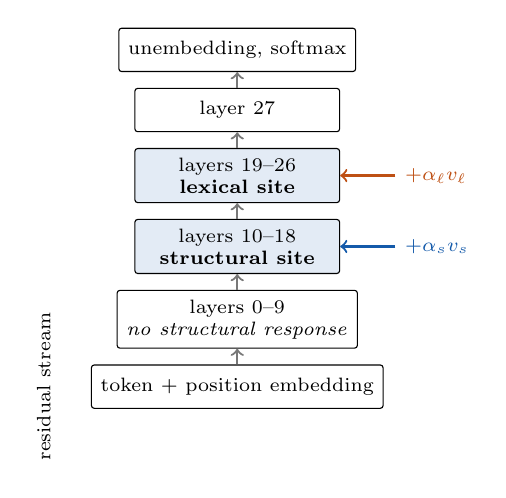
\begin{tikzpicture}[font=\small,node distance=2mm]
  \tikzset{
    blk/.style={draw,rounded corners=1pt,minimum width=2.6cm,minimum height=5.5mm,
                align=center,font=\scriptsize},
    inj/.style={draw,fill=cstruct!12,rounded corners=1pt,minimum width=2.6cm,
                minimum height=5.5mm,align=center,font=\scriptsize}
  }
  \node[blk] (e) {token + position embedding};
  \node[blk,above=of e] (l1) {layers 0--9\\\textit{no structural response}};
  \node[inj,above=of l1] (l2) {layers 10--18\\\textbf{structural site}};
  \node[inj,above=of l2] (l3) {layers 19--26\\\textbf{lexical site}};
  \node[blk,above=of l3] (l4) {layer 27};
  \node[blk,above=of l4] (u) {unembedding, softmax};

  \foreach \a/\b in {e/l1,l1/l2,l2/l3,l3/l4,l4/u}
    \draw[->,thick,cgrey] (\a) -- (\b);

  % injection arrows
  \node[right=7mm of l2,font=\scriptsize,cstruct] (vs) {$+\alpha_s v_s$};
  \node[right=7mm of l3,font=\scriptsize,clex] (vl) {$+\alpha_\ell v_\ell$};
  \draw[->,thick,cstruct] (vs) -- (l2);
  \draw[->,thick,clex] (vl) -- (l3);

  \node[left=6mm of e,font=\scriptsize,align=center,rotate=90,anchor=center]
    {residual stream};
\end{tikzpicture}
\caption{Injection sites in the 28-layer stack. Each decoder layer adds to the
residual stream; steering adds one more term. The two depth bands are the
measured response regions from Section~\ref{sec:sweep}, not a design choice.}
\label{fig:stack}
\end{figure}

Injection is implemented with PyTorch forward hooks on the decoder-layer
modules. A hook receives the layer output and may return a replacement. The
recorder counterpart reads the same tensor and returns \code{None}, which leaves
the output untouched.

Position selection matters. With a key-value cache, prefill is one call carrying
the whole prompt and each decode step carries one token. Without a cache, every
call carries the whole sequence. Injecting on generated tokens only therefore
cannot be decided by counting calls; the implementation compares the current
sequence length against the remembered prompt length.

\paragraph{Setup.} Apple M4 Max, 128\,GB unified memory, bfloat16 on the MPS
backend. Model \code{Llama-3.2-3B-Instruct}: 28 layers, hidden size 3072.
Faithfulness scoring uses \code{roberta-large-mnli}.

Weights are fetched with \code{aria2c} at 16 connections per file and 4 files
concurrently, because the Hugging Face client opens one connection per file.
One access detail cost time: \code{meta-llama} gates Llama-3.2 behind a licence
separate from Llama-3.1, so a token can read Llama-3.1 and receive HTTP 403 on
every Llama-3.2 file while repository \emph{metadata} stays public. Listing files
succeeds and downloading fails. The ungated mirror
\code{unsloth/Llama-3.2-3B-Instruct} carries byte-identical bfloat16 shards
(4\,965\,799\,096 and 1\,459\,729\,952 bytes), verified against the gated
repository's own metadata.

\section{Extracting vectors}

Three estimators produce the same output shape, so the sweep can compare them.

\paragraph{Instruction difference.} Take a corpus of complex texts. For each,
run two forward passes whose prompts differ only in one instruction, and average
the difference of the pooled hidden state:
\begin{equation}
v_l = \frac{1}{N}\sum_{i=1}^{N}
      \bigl[h_l(x_i \oplus q) - h_l(x_i \oplus \bar q)\bigr].
\label{eq:idiff}
\end{equation}
Here $q$ is the axis instruction and $\bar q$ its contrast. Both prompts end in
the same generation-prompt token, so pooling the last position isolates the
instruction's effect on the state from which the model begins to answer.

The choice of $\bar q$ decides whether this works. Setting $\bar q = \emptyset$
fails: the difference is then dominated by the prompt being longer, not by what
the instruction said. Measured on 256 texts, the structural and lexical vectors
came out at mean absolute cosine $0.983$ under that contrast. Replacing
$\bar q$ with an axis-matched placebo of comparable length cancels the shared
component. The structural pair is ``Use short, simple sentences with one idea
each'' against ``Keep the original sentence structure and sentence length exactly
as they are''; the lexical pair varies wording and holds structure fixed.

\paragraph{Contrastive activation addition.} Given aligned pairs,
\begin{equation}
v_l = \mathbb{E}[h_l(\text{simple})] - \mathbb{E}[h_l(\text{complex})].
\end{equation}
Pairs are generated by the model itself, prompted once per axis.

\paragraph{Difference PCA.} The leading right singular vector of the centred
per-pair differences, sign-aligned to the mean difference. This detects a mean
dragged by outliers.

\subsection{Scaling strength by depth}

Residual norms grow with depth. Figure~\ref{fig:refnorm} plots the measured mean
activation norm per layer: $1.60$ at layer 0 rising to $52.04$ at layer 27, a
factor of 33. A raw $\alpha$ of $1.0$ is therefore a small nudge early and an
overwrite late, and a layer sweep on raw $\alpha$ compares nothing.

Each bank stores those norms and injects
\begin{equation}
\alpha \cdot \frac{v_l}{\lVert v_l \rVert} \cdot \bar n_l ,
\qquad
\bar n_l = \mathbb{E}\bigl[\lVert h_l \rVert\bigr],
\label{eq:scale}
\end{equation}
so $\alpha$ means a fraction of a typical hidden-state magnitude and is
comparable across depth. Every $\alpha$ in this report is that quantity.

\begin{figure}[t]
\centering
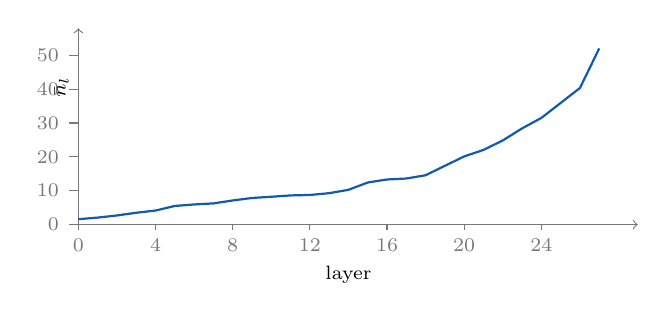
\begin{tikzpicture}[x=0.245cm,y=0.043cm,font=\scriptsize]
  \draw[->,cgrey] (0,0) -- (29,0);
  \draw[->,cgrey] (0,0) -- (0,58);
  \foreach \x in {0,4,8,12,16,20,24} \draw[cgrey] (\x,0) -- (\x,-1.5) node[below]{\x};
  \foreach \y in {0,10,20,30,40,50} \draw[cgrey] (0,\y) -- (-0.5,\y) node[left]{\y};
  \node[below=4mm of {(14,0)},font=\scriptsize] {layer};
  \node[rotate=90,above=5mm of {(0,29)},anchor=south,font=\scriptsize] {$\bar n_l$};
  \draw[thick,cstruct] plot coordinates {
    (0,1.60)(1,2.07)(2,2.70)(3,3.50)(4,4.15)(5,5.51)(6,5.95)(7,6.26)(8,7.13)
    (9,7.86)(10,8.22)(11,8.62)(12,8.75)(13,9.28)(14,10.27)(15,12.43)(16,13.33)
    (17,13.61)(18,14.58)(19,17.37)(20,20.13)(21,22.06)(22,24.86)(23,28.42)
    (24,31.51)(25,35.93)(26,40.35)(27,52.04)};
\end{tikzpicture}
\caption{Mean residual norm by layer, over 256 texts. The 33-fold growth is why
$\alpha$ is expressed as a fraction of $\bar n_l$ rather than in absolute units.}
\label{fig:refnorm}
\end{figure}

\section{A defect that faked a result}
\label{sec:mps}

The recorder pooled a hidden state and moved it to host memory in one call:
\code{pooled.detach().to("cpu", torch.float32)}. On the MPS backend, a combined
device-and-dtype cast of a half-precision tensor \emph{view} ignores the view's
storage offset and copies from the base of the allocation.

The failure is narrow, which is why it survived review. It fires only when the
view reports itself contiguous. For \code{hidden[:,-1,:]} that means batch size
one, and batch size one was the only shape the recorder ever produced. A batched
view is strided, takes a gather path, and is unaffected. Figure~\ref{fig:offset}
shows the mechanism.

\begin{figure}[t]
\centering
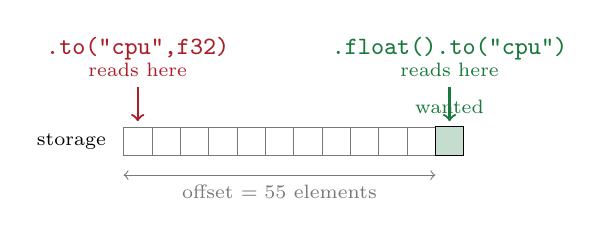
\begin{tikzpicture}[font=\scriptsize,x=0.36cm,y=0.36cm]
  % storage strip
  \foreach \i in {0,...,11}{
    \draw[cgrey,very thin] (\i,0) rectangle (\i+1,1);
  }
  \foreach \i in {11}{
    \draw[fill=cgood!25] (\i,0) rectangle (\i+1,1);
  }
  \node[left=1mm of {(0,0.5)}] {storage};
  \draw[<->,cgrey] (0,-0.7) -- (11,-0.7) node[midway,below]{offset $=55$ elements};
  \node[above=0.5mm of {(11.5,1)},cgood] {wanted};
  \draw[->,thick,cbad] (0.5,2.4) -- (0.5,1.2);
  \node[above=0.5mm of {(0.5,2.3)},cbad,align=center] {\code{.to("cpu",f32)}\\reads here};
  \draw[->,thick,cgood] (11.5,2.4) -- (11.5,1.2);
  \node[above=0.5mm of {(11.5,2.3)},cgood,align=center] {\code{.float().to("cpu")}\\reads here};
\end{tikzpicture}
\caption{The view \code{x[:,-1,:]} begins 55 elements into its allocation. A
fused device-and-dtype cast discards that offset. Casting dtype first allocates a
fresh contiguous tensor at offset zero, so the host copy is correct.}
\label{fig:offset}
\end{figure}

A minimal reproduction uses no project code. With
\code{x = arange(60).reshape(1,12,5)} as bfloat16 on MPS,
\code{x[:,-1,:].to('cpu', torch.float32)} yields $2.362\times10^{-41}$ where
\code{x[:,-1,:].float().to('cpu')} yields $55.0$.

The consequences were systematic, and they looked like a finding rather than a
fault. Table~\ref{tab:mpsfix} lists them. Recorded norms were identical at every
layer, which no residual stream is. Eleven layer-pairs held bit-identical
3072-dimensional mean vectors over 256 texts. The structural and lexical vectors
sat at cosine $0.983$ at every layer, which reads as ``the model encodes a single
simplify direction''. That conclusion was drawn and was wrong.

\begin{table}[t]
\centering
\small
\begin{tabular}{lrr}
\toprule
Quantity & Defective & Fixed \\
\midrule
$\lVert h \rVert$ recorded, layer 0  & 54.69 & 1.57 \\
$\lVert h \rVert$ recorded, layer 14 & 55.10 & 12.28 \\
$\lVert h \rVert$ recorded, layer 27 & 55.14 & 45.21 \\
cosine vs.\ ground truth             & 0.02  & 1.000000 \\
bit-identical layer pairs            & 11    & 0 \\
axis cosine, mean absolute           & 0.983 & 0.223 \\
\bottomrule
\end{tabular}
\caption{Before and after casting dtype before device. Ground truth is an
independent capture through a separate hook.}
\label{tab:mpsfix}
\end{table}

Two lessons are worth separating. The arithmetic error was in a one-line utility
with no branching. The detection required comparing the recorder against an
independent capture of the same tensor, because every internal consistency check
passed: shapes, dtypes, and finite values were all correct.

\section{Other defects}

Table~\ref{tab:defects} lists the remaining defects found by targeted testing.
None was reported by static analysis. A linter was run over the codebase
afterwards and produced 4 errors and 56 warnings, all of which were verified as
false positives: its \code{assert-tuple} rule flags the correct
\code{assert cond, (a, b)} two-argument form, and its bare-except rule flags
clauses that specify a type.

\begin{table*}[t]
\centering
\small
\begin{tabular}{p{3.4cm}p{6.2cm}p{6.2cm}}
\toprule
Site & Mechanism & Consequence \\
\midrule
Prefill detection & Prefill inferred from a call counter; decode assumed a
sequence length of one & With \code{use\_cache=False} the generated-tokens-only
mode injected into every prompt position \\
Hook state reset & Counter reset on block entry, not per generation & Only the
first generation inside one \code{with} block was correct; later ones either
stopped steering or steered the prompt \\
Position validation & \code{positions} was an unchecked string literal &
\code{"prompt\_alll"} silently behaved as \code{"all"} \\
Gemma-3n layer output & \code{altup} returns
\code{[streams, batch, seq, hidden]}, rank 4 & Three-dimensional indexing
addressed batch instead of sequence on the whole Gemma path \\
Prompt mean pooling & Attention mask never reaches a forward hook & Averaged
over left padding \\
Local model resolution & Directory judged complete once \code{config.json}
existed & Truncated shards were loaded; a later fix matched its own
\code{.aria2} \emph{directory} and refused every load \\
Pad token & \code{pad\_token\_id or eos\_token\_id} & Gemma-3n has pad id 0, so
the falsy test replaced it with the end-of-sequence token \\
Perplexity masking & Prompt and prompt-plus-output tokenised separately & BPE
merges across the join shifted every label; masking now uses the shared prefix \\
Hard-word rate & \code{textstat.difficult\_words} counts \emph{distinct} hard
words & Reusing one hard term read as a 50\% lexical simplification. Two 15-word
texts scored 2 against 4 deduplicated and 4 against 4 per token \\
\bottomrule
\end{tabular}
\caption{Defects found by differential testing. Each altered a measured
quantity.}
\label{tab:defects}
\end{table*}

\section{Independent dials}

Two unit vectors $a$ and $b$ with $a\cdot b = c$ are made orthogonal by
Gram-Schmidt in one direction. Applying it in both directions does not
orthogonalise the pair. Writing $a' = a - cb$ and $b' = b - ca$,
\begin{equation}
\frac{a'\cdot b'}{\lVert a'\rVert\,\lVert b'\rVert}
 = \frac{c - c^2 - c^2 + c^3}{1 - c^2} = -c .
\label{eq:gs}
\end{equation}
The correlation changes sign and keeps its magnitude. Measured on real banks,
$+0.500$ became $-0.504$, matching Equation~\ref{eq:gs} to three decimals.

L\"owdin symmetric orthogonalisation is the correct operation. With $V$ the
matrix of axis vectors and $G = V^\top V$ its Gram matrix,
\begin{equation}
V' = V G^{-1/2}
\label{eq:lowdin}
\end{equation}
gives an exactly orthonormal set, closest to $V$ in Frobenius norm, treating
every axis alike. Verified residual cosine is $2\times10^{-7}$ on synthetic input
and $1.02\times10^{-7}$ on the real banks. A small eigenvalue of $G$ signals that
the axes were nearly collinear at that layer and the orthogonal directions are
close to arbitrary, so the smallest eigenvalue is reported.

\section{Metrics}
\label{sec:metrics}

Four families of measurement are needed, and the interaction between them is the
part that is easy to get wrong.

\paragraph{Readability.} Flesch-Kincaid grade level, Flesch Reading Ease,
Dale-Chall hard-word rate counted per token, words per sentence, clauses per
sentence, syllables per word.

\paragraph{Faithfulness.} Bidirectional natural language inference. One
direction is insufficient. Requiring only that the source entails the output
rewards deleting facts, because a shorter claim is trivially entailed. Requiring
only the reverse rewards inventing detail. Both are required. Scoring is per
sentence so a single dropped fact appears in the minimum rather than washing out
of an average.

\paragraph{Fluency.} Perplexity of the output under the same model with no hook
attached. The reference model must be untouched for the number to mean anything.

\paragraph{Reference-based quality.} SARI, over $n$-grams of order 1 to 4,
averaging additions, retentions and deletions. Our implementation agrees with the
reference implementation to $2.84\times10^{-14}$ over 3000 randomised cases.

\subsection{Gate simplicity on fluency}

Every simplicity metric is maximised by broken text. Collapsed output such as
\code{"The,, a a the the the"} contains no difficult words and no long sentences.
One sweep cell recorded a 91\% reduction in hard-word rate with every output
destroyed. Simplicity is therefore credited only on outputs that pass a
degeneracy check, and the number of survivors is reported alongside.

\subsection{Why the check is narrow}

Genuine simplification is statistically similar to degeneration. The valid
sentence group \emph{The cell makes energy. The cell uses energy. The cell needs
energy.} has a type-token ratio of $0.5$ and 45\% of its bigrams repeated. Those
are the same signals a broken generation produces, and that text is exactly what
the system is meant to output.

Two plausible backstops do not work, and both were tested rather than assumed.

Perplexity does not detect repetition. Repetition is low-entropy, so a loop is
cheaper under the model than ordinary prose. The broken fragment
\emph{organe-cepted control-cepted control-cepted contr} scored $18.8$ while the
valid repetitive group above scored $37.0$. Any threshold catching the first
rejects the second. Perplexity guards high-entropy breakage only.

Dictionary lookup does not work either. The system word list is Webster's Second,
which predates most scientific vocabulary, so \emph{mitochondrion} reads as
out-of-vocabulary. Valid academic prose scored $0.22$ out-of-vocabulary against
$0.27$ for the broken fragment.

What remains is a rule set that fires only on text that is not language.
Figure~\ref{fig:gate} shows the order of evaluation. Immediate $n$-gram
repetition is the discriminating signal, with two corrections. It must be
computed per sentence, because a flat token list cannot see sentence boundaries
and the ordinary pair \emph{\dots sleet and freezing rain. Freezing rain can be
heavy\dots} then reads as a repeating bigram. It must also exclude loops built
from function words, because \emph{on and on and on} and \emph{row after row
after row} are English while \emph{cepted control cepted control} is not, unless
the phrase repeats three or more times. The final rule set produces no false
positives and no false negatives across 13 hand-built cases and 24 real
paragraphs.

\begin{figure}[t]
\centering
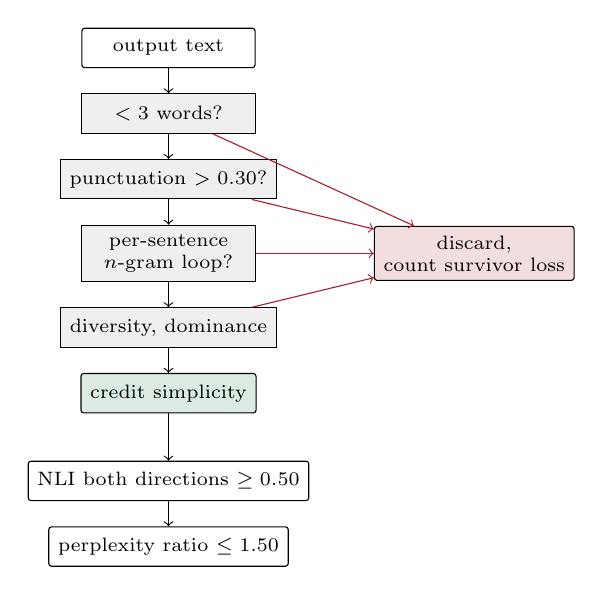
\begin{tikzpicture}[font=\scriptsize,node distance=3.2mm,
  st/.style={draw,rounded corners=1pt,align=center,minimum height=5mm,
             minimum width=2.2cm},
  dc/.style={draw,align=center,minimum height=5mm,minimum width=2.2cm,
             fill=cgrey!12}]
  \node[st] (o) {output text};
  \node[dc,below=of o] (d1) {$<3$ words?};
  \node[dc,below=of d1] (d2) {punctuation $>0.30$?};
  \node[dc,below=of d2] (d3) {per-sentence\\$n$-gram loop?};
  \node[dc,below=of d3] (d4) {diversity, dominance};
  \node[st,below=of d4,fill=cgood!15] (ok) {credit simplicity};
  \node[st,right=1.5cm of d3,fill=cbad!15] (rej) {discard,\\count survivor loss};
  \foreach \a/\b in {o/d1,d1/d2,d2/d3,d3/d4,d4/ok}
    \draw[->] (\a) -- (\b);
  \foreach \n in {d1,d2,d3,d4} \draw[->,cbad] (\n) -- (rej);
  \node[st,below=6mm of ok] (nli) {NLI both directions $\ge 0.50$};
  \node[st,below=of nli] (ppl) {perplexity ratio $\le 1.50$};
  \draw[->] (ok) -- (nli); \draw[->] (nli) -- (ppl);
\end{tikzpicture}
\caption{Gate order. Degeneracy is checked before any simplicity metric is
credited, because broken text maximises all of them.}
\label{fig:gate}
\end{figure}

\subsection{FKGL fails on sentences}

Flesch-Kincaid is a passage-level formula. At single-sentence length it is
dominated by syllables per word and by the sentence's own length, so it rewards
padding and penalises concision. This is not a small effect. A faithful 17-word
paraphrase with NLI $0.990$ against its source scored $14.3$, while a 60-word
rewrite that invented three entities and scored NLI $0.090$ scored $7.0$.

The consequence for this project is direct: an early comparison used Flesch-Kincaid
to conclude that prompting outperformed steering. That comparison measured
padding. Sentence-level judgements belong to SARI and to the faithfulness gate.

\section{Data}

ASSET supplies 359 test and 2000 validation sentences with 10 human references
each. The 10 references are what makes SARI meaningful, so all are retained.

The estimation corpus is 256 texts drawn from a 665-item filtered pool of ASSET
validation sources. Disjointness from the test set is recomputed on every call
rather than trusted from the upstream split, so a stale cache cannot reintroduce
leakage. Passages come from a pool of 11\,854 paragraphs, of which 2 were dropped
for containing an ASSET sentence verbatim.

OneStopEnglish required care. The flat three-class datasets are not
index-aligned, although they appear to be. Content-overlap matching identified
the presumed partner for only 184, 186 and 187 of 189 pairs across the three
level combinations, and index 53 pairs a skydiving article with a royal birth. A
duplicated elementary text shifts everything after it. Aligned triples were
instead taken from OneStopQA, which carries explicit title, paragraph and level
keys, yielding 162 aligned paragraph triples.

\section{Layer and strength sweep}
\label{sec:sweep}

The full grid of 28 layers, 8 strengths, 2 axes and 48 texts is roughly a day of
wall clock. It is split. Stage 1 scans every layer at two coarse strengths with
12 texts. Stage 2 runs the full strength grid on surviving layers and adds NLI.

Effects are measured against each text's own \emph{unsteered rewrite}, not
against the source. Both are rewrites, so the difference isolates what steering
did from what asking for a rewrite did.

\subsection{Depth}

Figure~\ref{fig:depth} plots stage-1 results. The structural response is confined
to layers 10 to 18 and is absent on either side. The lexical response is smaller
and spread, with local maxima at layers 16 and 23.

\begin{figure}[t]
\centering
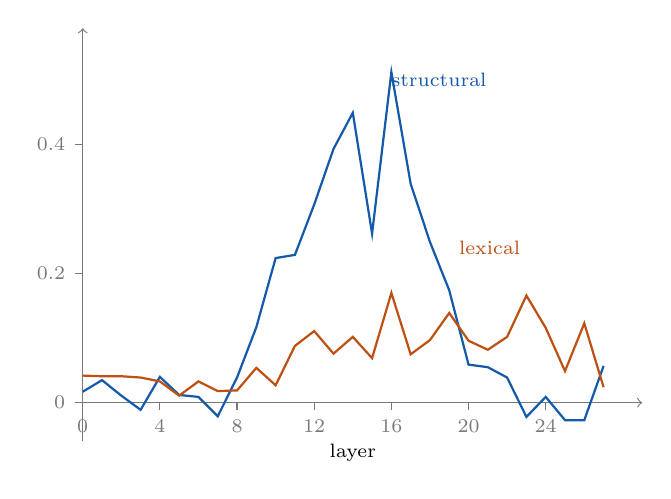
\begin{tikzpicture}[x=0.245cm,y=8.2cm,font=\scriptsize]
  \draw[->,cgrey] (0,0) -- (29,0);
  \draw[->,cgrey] (0,-0.06) -- (0,0.58);
  \draw[cgrey,very thin,dashed] (0,0) -- (28,0);
  \foreach \x in {0,4,8,12,16,20,24} \draw[cgrey] (\x,0) -- (\x,-0.012) node[below]{\x};
  \foreach \y in {0,0.2,0.4} \draw[cgrey] (0,\y) -- (-0.4,\y) node[left]{\y};
  \node[below=4mm of {(14,0)}] {layer};
  \draw[thick,cstruct] plot coordinates {
    (0,0.017)(1,0.035)(2,0.011)(3,-0.011)(4,0.040)(5,0.012)(6,0.009)(7,-0.021)
    (8,0.039)(9,0.117)(10,0.224)(11,0.229)(12,0.307)(13,0.393)(14,0.449)
    (15,0.262)(16,0.512)(17,0.339)(18,0.249)(19,0.174)(20,0.059)(21,0.055)
    (22,0.039)(23,-0.022)(24,0.009)(25,-0.027)(26,-0.027)(27,0.057)};
  \draw[thick,clex] plot coordinates {
    (0,0.042)(1,0.041)(2,0.041)(3,0.039)(4,0.033)(5,0.011)(6,0.033)(7,0.018)
    (8,0.019)(9,0.054)(10,0.027)(11,0.088)(12,0.111)(13,0.076)(14,0.102)
    (15,0.069)(16,0.170)(17,0.075)(18,0.097)(19,0.139)(20,0.096)(21,0.082)
    (22,0.102)(23,0.166)(24,0.116)(25,0.049)(26,0.123)(27,0.024)};
  \node[cstruct,anchor=west,font=\scriptsize] at (15.5,0.50) {structural};
  \node[clex,anchor=west,font=\scriptsize] at (19,0.24) {lexical};
\end{tikzpicture}
\caption{Stage-1 own-axis effect by layer, as a fractional reduction against the
unsteered rewrite, taking the better of the two coarse strengths. Structural
effect is confined to layers 10 to 18. Values at layers 14 and 16 rest on 9 and
8 surviving outputs of 12 and are not used for selection.}
\label{fig:depth}
\end{figure}

Axis entanglement depends strongly on the estimator. Figure~\ref{fig:cos} plots
per-layer cosine for both. Instruction difference gives mean absolute cosine
$0.223$; contrastive activation addition gives $0.673$, reaching $0.976$ at layer
1.

The reason is structural, not a data-quality problem. Inspection confirms the
generated pairs are well isolated: for a source about Gothic architecture, the
lexical rewrite preserved sentence structure and substituted
\emph{churches}, \emph{monasteries} and \emph{village churches}, while the
structural rewrite split the sentence into three. Contrastive addition
nevertheless conflates the axes because it contrasts an output against its
source, and both axis outputs share the property being varied, namely being
simpler than the source. Differencing two instructions that differ along one axis
cancels that shared component instead.

\begin{figure}[t]
\centering
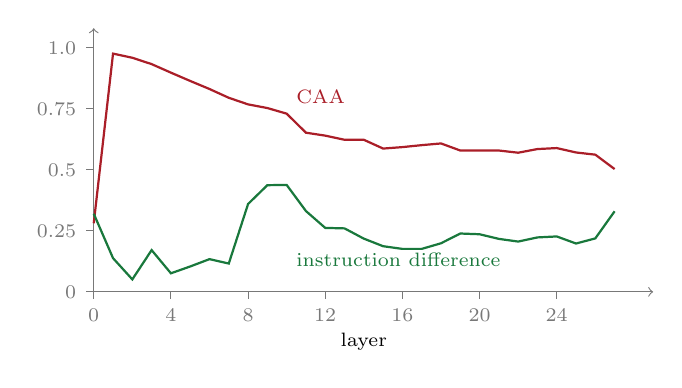
\begin{tikzpicture}[x=0.245cm,y=3.1cm,font=\scriptsize]
  \draw[->,cgrey] (0,0) -- (29,0);
  \draw[->,cgrey] (0,0) -- (0,1.08);
  \foreach \x in {0,4,8,12,16,20,24} \draw[cgrey] (\x,0) -- (\x,-0.03) node[below]{\x};
  \foreach \y in {0,0.25,0.5,0.75,1.0} \draw[cgrey] (0,\y) -- (-0.4,\y) node[left]{\y};
  \node[below=4mm of {(14,0)}] {layer};
  \draw[thick,cbad] plot coordinates {
    (0,0.281)(1,0.976)(2,0.959)(3,0.933)(4,0.898)(5,0.864)(6,0.831)(7,0.795)
    (8,0.768)(9,0.753)(10,0.730)(11,0.652)(12,0.640)(13,0.623)(14,0.623)
    (15,0.587)(16,0.593)(17,0.601)(18,0.608)(19,0.579)(20,0.579)(21,0.579)
    (22,0.570)(23,0.585)(24,0.589)(25,0.571)(26,0.562)(27,0.503)};
  \draw[thick,cgood] plot coordinates {
    (0,0.320)(1,0.138)(2,0.051)(3,0.171)(4,0.076)(5,0.104)(6,0.134)(7,0.116)
    (8,0.360)(9,0.437)(10,0.438)(11,0.331)(12,0.262)(13,0.260)(14,0.218)
    (15,0.187)(16,0.176)(17,0.176)(18,0.199)(19,0.239)(20,0.236)(21,0.217)
    (22,0.206)(23,0.223)(24,0.227)(25,0.198)(26,0.219)(27,0.330)};
  \node[cbad,anchor=west] at (10,0.80) {CAA};
  \node[cgood,anchor=west] at (10,0.13) {instruction difference};
\end{tikzpicture}
\caption{Absolute cosine between the structural and lexical vectors, per layer,
by estimator. Lower is more separable.}
\label{fig:cos}
\end{figure}

\subsection{Strength}

Figure~\ref{fig:alpha} plots stage-2 response. Three properties matter.

Response is not monotone. Structural effect at layer 17 peaks at $+0.339$ at
$\alpha = 1.0$ and falls to $+0.027$ at $\alpha = 1.25$ as degeneration begins.
Any search over $\alpha$ must therefore bisect inside a bracket verified to be
both monotone and gate-passing, never assume monotonicity globally.

The sign is correct. At $\alpha = -1.0$ the structural vector at layer 17
\emph{lengthens} sentences by 60\%, own-axis effect $-0.598$. A direction that
simplified in both directions would indicate an artifact rather than a concept.

The two axes have different usable ranges. Structural saturates and then
collapses between $1.0$ and $1.25$, while lexical is still climbing at $1.5$.
Stage 1 sampled only $0.5$ and $1.0$ and consequently reported the lexical axis
as weak; that was a property of the grid, not of the axis.

\begin{figure*}[t]
\centering
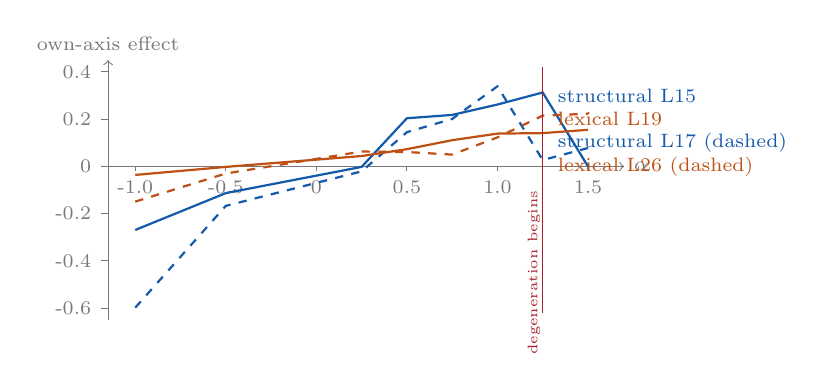
\begin{tikzpicture}[x=2.3cm,y=3.0cm,font=\scriptsize]
  \draw[->,cgrey] (-1.15,0) -- (1.7,0) node[right]{$\alpha$};
  \draw[->,cgrey] (-1.15,-0.65) -- (-1.15,0.45) node[above]{own-axis effect};
  \draw[cgrey,very thin,dashed] (-1.15,0) -- (1.6,0);
  \foreach \x in {-1.0,-0.5,0,0.5,1.0,1.5} \draw[cgrey] (\x,0) -- (\x,-0.02) node[below]{\x};
  \foreach \y in {-0.6,-0.4,-0.2,0,0.2,0.4} \draw[cgrey] (-1.15,\y) -- (-1.19,\y) node[left]{\y};
  \draw[thick,cstruct] plot coordinates {(-1.0,-0.269)(-0.5,-0.113)(0.25,-0.002)(0.5,0.204)(0.75,0.218)(1.0,0.262)(1.25,0.313)(1.5,-0.000)};
  \draw[thick,cstruct,dashed] plot coordinates {(-1.0,-0.598)(-0.5,-0.167)(0.25,-0.021)(0.5,0.145)(0.75,0.201)(1.0,0.339)(1.25,0.027)(1.5,0.078)};
  \draw[thick,clex] plot coordinates {(-1.0,-0.036)(-0.5,-0.002)(0.25,0.044)(0.5,0.073)(0.75,0.111)(1.0,0.139)(1.25,0.141)(1.5,0.155)};
  \draw[thick,clex,dashed] plot coordinates {(-1.0,-0.149)(-0.5,-0.030)(0.25,0.063)(0.5,0.061)(0.75,0.050)(1.0,0.123)(1.25,0.215)(1.5,0.223)};
  \node[cstruct,anchor=west] at (1.28,0.30) {structural L15};
  \node[cstruct,anchor=west] at (1.28,0.10) {structural L17 (dashed)};
  \node[clex,anchor=west] at (1.28,0.20) {lexical L19};
  \node[clex,anchor=west] at (1.28,0.00) {lexical L26 (dashed)};
  % degeneration band
  \draw[cbad,very thin] (1.25,-0.62) -- (1.25,0.42);
  \node[cbad,anchor=south,rotate=90,font=\tiny] at (1.29,-0.45) {degeneration begins};
\end{tikzpicture}
\caption{Stage-2 strength response. Negative $\alpha$ reverses the effect, which
confirms the vectors encode the intended concepts. The structural curves turn
over past $\alpha = 1.0$; the lexical curves are still rising at $1.5$.}
\label{fig:alpha}
\end{figure*}

\subsection{A metric that rewarded inaction}

Selectivity was defined as own-axis effect minus the absolute cross-axis effect.
A cell with no effect at all scores $0 - 0 = 0$, which outranks a cell with a
large own-axis effect and a moderate cross-axis one. The first stage-1 report
consequently named layer 4 the best lexical site at selectivity $+0.002$, where
both effects were noise. Selection now requires a minimum own-axis effect of
$0.05$ before selectivity is considered.

Table~\ref{tab:best} lists the best cells under the corrected rule, at zero
degeneration and with the faithfulness gate passing on at least 75\% of items.

\begin{table}[t]
\centering
\small
\begin{tabular}{llrrrr}
\toprule
Axis & Site & Own & Other & NLI & Gate \\
\midrule
structural & L17, 1.00 & $+0.339$ & $+0.070$ & 0.701 & 75\% \\
structural & L15, 0.75 & $+0.218$ & $-0.014$ & 0.765 & 83\% \\
structural & L15, 0.50 & $+0.204$ & $-0.010$ & \textbf{0.873} & \textbf{100\%} \\
lexical    & L19, 1.00 & $+0.139$ & $-0.105$ & 0.830 & 92\% \\
lexical    & L26, 1.00 & $+0.123$ & $-0.178$ & 0.749 & 83\% \\
lexical    & L19, 0.75 & $+0.111$ & $-0.021$ & 0.853 & 92\% \\
\bottomrule
\end{tabular}
\caption{Best cells by own-axis effect. Structural is both stronger and more
selective: at L15 with $\alpha=0.5$ it moves its own axis by $+0.204$ while
disturbing the other by $-0.010$. Lexical always lengthens sentences.}
\label{tab:best}
\end{table}

\section{Calibration}

Mapping $\alpha$ onto a named reading level requires searching for the $\alpha$
that reaches a target Flesch-Kincaid grade subject to the gates. No target was
reachable. Gate-passing grade spans $12.19$ to $14.76$ for the structural axis
and $13.84$ to $14.76$ for the lexical axis, against a baseline of $14.76$ and
targets of 4, 6 and 8.

Pushing harder does not help, because there is no range left to spend. At
$\alpha = 1.389$ the grade \emph{rises} to $15.77$ with NLI $0.385$ and 25\% of
outputs degenerate. At $\alpha = 2.0$ the grade is $21.61$, NLI $0.153$, and 75\%
are degenerate. The search reports this as unreachable rather than returning the
closest gate-violating point.

\section{Layer bands}

Spreading a smaller $\alpha$ across a band of layers is the obvious way to widen
the range. It buys little and costs stability.
Table~\ref{tab:bands} gives the measurements. The best zero-degeneration band
reaches grade $12.79$ against $13.74$ for the best single layer, an improvement
of about one grade level. The cliff becomes far steeper: the same band moves from
0\% to 83\% degenerate between $\alpha = 0.1$ and $0.2$. Bands across both axes
collapse entirely. Single-layer injection with a calibrated $\alpha$ remains the
better operating point.

\begin{table}[t]
\centering
\small
\begin{tabular}{lrrrr}
\toprule
Configuration & FKGL & w/sent & NLI & Degen \\
\midrule
unsteered              & 16.80 & 27.5 & --    & 0\% \\
prompt-only            & \textbf{7.91} & 17.1 & \textbf{0.161} & 0\% \\
L15, $\alpha{=}0.75$   & 13.74 & 21.6 & 0.691 & 0\% \\
L12--18, $\alpha{=}0.1$ & 13.64 & 20.2 & \textbf{0.847} & 0\% \\
L10--19, $\alpha{=}0.1$ & \textbf{12.79} & 19.6 & 0.595 & 0\% \\
L12--18, $\alpha{=}0.2$ & 10.02 & 11.6 & 0.834 & \textbf{83\%} \\
\bottomrule
\end{tabular}
\caption{Band probe, 12 held-out texts. Prompt-only reaches the lowest grade and
fails the faithfulness gate by a wide margin.}
\label{tab:bands}
\end{table}

\section{Evaluation}

Table~\ref{tab:eval} reports all six variants on the ASSET test set at $n=32$,
with structural steering at layer 15 and $\alpha = 0.75$ and lexical steering at
layer 19 and $\alpha = 1.0$.

\begin{table*}[t]
\centering
\small
\begin{tabular}{lrrrrrrrr}
\toprule
Variant & FKGL & w/sent & hard & NLI & Gate & PPL ratio & SARI & Degen \\
\midrule
unsteered             & 12.49 & 20.36 & 0.345 & 0.875 & 90.6\% & 1.00 & 45.44 & 0\% \\
prompted              & \textbf{6.78} & 15.15 & 0.161 & 0.431 & 40.6\% & 3.64 & 40.40 & 0\% \\
steered structural    & 10.15 & 16.62 & 0.323 & 0.795 & 81.2\% & 1.31 & \textbf{45.87} & \textbf{0\%} \\
steered lexical       & 12.30 & 21.84 & 0.324 & 0.845 & 90.6\% & 1.20 & 44.07 & 0\% \\
steered dual          & 13.72 & 30.85 & 0.234 & 0.579 & 50.0\% & 2.02 & 41.17 & 34.4\% \\
prompted + steered    & 5.32 & 15.39 & 0.095 & 0.225 & 15.6\% & 4.74 & 31.94 & 65.6\% \\
\bottomrule
\end{tabular}
\caption{ASSET test, $n=32$, 10 references per item. Prompting reaches the lowest
grade level and the worst faithfulness. Perplexity ratio above 1.50 fails the
fluency gate.}
\label{tab:eval}
\end{table*}

Aggregate means can hide item-level variance, so every comparison is paired
per item. Figure~\ref{fig:forest} plots mean SARI difference against the
unsteered baseline with 95\% confidence intervals.

\begin{figure}[t]
\centering
\begin{tikzpicture}[x=0.155cm,y=0.75cm,font=\scriptsize]
  \draw[cgrey,dashed] (0,-0.4) -- (0,5.4);
  \draw[->,cgrey] (-19,-0.4) -- (11,-0.4) node[right]{$\Delta$SARI};
  \foreach \x in {-15,-10,-5,0,5,10} \draw[cgrey] (\x,-0.4) -- (\x,-0.55) node[below]{\x};
  % rows: y, lo, mean, hi, label, colour
  \foreach \y/\lo/\m/\hi/\lab/\c in {
    5/-1.75/0.43/2.61/{structural}/cgood,
    4/-3.29/-1.37/0.55/{lexical}/cgrey,
    3/-8.13/-5.04/-1.96/{prompted}/cbad,
    2/-7.13/-4.27/-1.41/{dual}/cbad,
    1/-17.42/-13.50/-9.58/{prompted+steered}/cbad}{
      \draw[\c,thick] (\lo,\y) -- (\hi,\y);
      \draw[\c,thick] (\lo,\y-0.1) -- (\lo,\y+0.1);
      \draw[\c,thick] (\hi,\y-0.1) -- (\hi,\y+0.1);
      \filldraw[\c] (\m,\y) circle (1.6pt);
      \node[anchor=west,font=\tiny] at (11.5,\y) {\lab};
  }
\end{tikzpicture}
\caption{Paired per-item SARI difference against no intervention, 95\% intervals,
$n=32$. Structural steering is a tie: its interval spans zero. The three lower
rows are significantly worse than no intervention. Only structural steering fails
to be worse.}
\label{fig:forest}
\end{figure}

Three results follow.

Structural steering beats prompt-only significantly. On the same paired basis,
SARI improves by $+5.47$ (CI $+2.45$ to $+8.49$, 23 wins against 9) and
faithfulness by $+0.36$ (CI $+0.23$ to $+0.50$, 27 against 5).

Structural steering does not beat doing nothing on SARI. The difference is
$+0.43$ with an interval spanning zero. What it does is reduce sentence length
18\% and grade level 19\% at no measurable cost in SARI and none in faithfulness
($-0.08$, CI $-0.21$ to $+0.05$). That satisfies the requirement, which was to
simplify without changing meaning, not to improve on the source.

Prompting is significantly worse than no intervention, at $-5.04$ SARI with NLI
$0.431$ and a perplexity ratio of $3.64$.

\subsection{Output samples}

Table~\ref{tab:qual} shows why the faithfulness numbers diverge from the grade
levels. Prompting reaches a low grade by replacing content. In the second case it
substitutes an analogy for a statistic and drops the figure entirely.

\begin{table*}[t]
\centering
\small
\begin{tabular}{p{2.0cm}p{6.4cm}p{6.4cm}}
\toprule
& Case 1 & Case 2 \\
\midrule
Source &
Some academic journals do refer to Wikipedia articles, but are not elevating it
to the same level as traditional references. &
The aggregate income distribution is highly concentrated towards the top, with
the top 6.37\% earning roughly one third of all income. \\
\addlinespace
Prompt-only &
You might have noticed that some big schools and universities use Wikipedia
articles in their research\dots they don't think it's as good as other sources,
like books or articles from experts. &
Imagine you have a big jar of cookies, and you want to know how the cookies are
divided among the people\dots some groups have a lot more cookies than others. \\
& FKGL 7.0, NLI \textbf{0.090} & NLI \textbf{0.025} \\
\addlinespace
Steered, L15, $\alpha{=}0.75$ &
Some academic journals mention Wikipedia articles, but they do not consider them
equal to traditional references. &
The US income distribution is highly skewed towards the top, with the top 6.37\%
of earners holding about one-third of the country's total income. \\
& FKGL 14.3, NLI \textbf{0.990} & no-hallucination \textbf{0.63} \\
\bottomrule
\end{tabular}
\caption{Prompting invents universities, books and experts in case 1, and
replaces a statistic with a cookie-jar analogy in case 2, dropping the 6.37\%
figure. Steering retains both. Case 1 also shows the Flesch-Kincaid inversion:
the faithful output scores worse.}
\label{tab:qual}
\end{table*}

\section{Conclusions}

The two axes are separable directions at mean absolute cosine $0.223$ and they
respond at different depths, structure at layers 15 to 17 and vocabulary at
layers 19 to 26. The two-dial hypothesis holds as a statement about mechanism.

It does not hold as a product. The lexical dial is a SARI tie trending negative
at $-1.37$, it lengthens sentences as a side effect, and running both dials
together degenerates 34\% of outputs. The deliverable is one structural dial.

Steering is a modulator, not a replacement for a prompt. It cannot reach a target
reading level alone. Composition with a prompt is destructive rather than
additive: that variant is the worst tested, at $-13.50$ SARI and 66\% degenerate.

What steering does deliver is a continuous strength parameter that a prompt
cannot provide, and better meaning preservation than prompting at any setting
tested.

\section{Limitations}

Results are $n=32$ on one evaluation set. The contrastive and PCA estimators were
compared for axis separation only and never evaluated as steering vectors.
Passage-level results are $n \le 4$. Sentence-by-sentence passage simplification
is unreliable at this model size: on one paragraph it emitted the same sentence 6
times of 9 and invented a date not present in the source, so context is disabled
by default. Porting to Gemma-3n requires a fresh sweep, because its decoder
returns rank-4 output and the layer indices do not transfer.

\onecolumn
\appendix
\section*{Appendix: concepts used above}
\addcontentsline{toc}{section}{Appendix}
\begin{multicols}{2}
\small

\subsection*{Residual stream}
A decoder-only transformer keeps one vector per token position, of width equal to
the hidden size, here 3072. Each layer reads that vector, computes attention and
a feed-forward update, and \emph{adds} the result back. Nothing is overwritten.
The stream is therefore a running sum, and a direction added at layer $l$
persists through every later layer unless something cancels it. This is what
makes steering possible with a single addition.

\subsection*{Forward hook}
A callback attached to a module that fires after its forward pass, receiving the
module, its inputs and its output. Returning \code{None} leaves the output alone;
returning a tensor replaces it. Reading uses the first form, steering the second.
A hook that accidentally returns a value replaces the layer output with it, which
is a common source of confusing failures.

\subsection*{Activation steering and CAA}
Activation steering adds a fixed direction to internal activations at inference
to change behaviour, with no weight updates. Contrastive Activation Addition
obtains that direction as the mean difference in activations between paired
inputs that differ in the target property:
$v = \mathbb{E}[h^+] - \mathbb{E}[h^-]$. The assumption is that the property is
represented approximately linearly, so a single direction suffices.

\subsection*{bfloat16 and MPS}
bfloat16 keeps the 8 exponent bits of float32 and 8 mantissa bits, so it has the
dynamic range of float32 and about 3 significant decimal digits. MPS is PyTorch's
Metal backend for Apple GPUs. Reduced-precision paths on newer backends are
less exercised than CUDA equivalents, which is the class of defect described in
Section~\ref{sec:mps}.

\subsection*{Views, strides and storage offset}
A tensor is a view onto a flat allocation, described by a shape, a stride per
dimension, and a storage offset. \code{x[:,-1,:]} does not copy: it points into
the same allocation at offset $(\text{seq}-1)\times\text{hidden}$. A view is
called contiguous when its strides match a dense row-major layout. Contiguity
says nothing about the offset, and a copy routine that assumes offset zero for
contiguous inputs reads the wrong memory. That is the exact failure in
Section~\ref{sec:mps}.

\subsection*{Flesch-Kincaid grade level}
\[
0.39\frac{W}{S} + 11.8\frac{Y}{W} - 15.59
\]
for $W$ words, $S$ sentences and $Y$ syllables. It reports a US school grade.
Both terms grow with length, so on a single sentence the first term is the
sentence's own word count and the formula rewards splitting and padding. Flesch
Reading Ease is the same inputs on a 0 to 100 scale, higher being easier.

\subsection*{Dale-Chall}
Uses a list of about 3000 words familiar to fourth-grade readers. Anything off
the list is a hard word. The rate must be counted per token: counting distinct
hard words means a text reusing one hard term scores easier than one using
several, which inverts the measurement for technical prose that repeats its key
terms.

\subsection*{SARI}
The standard simplification metric, comparing system output against the source
\emph{and} multiple human references over $n$-grams of order 1 to 4. It scores
three operations. Additions are $n$-grams in the output but not the source,
credited when references also add them. Retentions are $n$-grams kept from the
source, credited when references keep them. Deletions are $n$-grams removed from
the source, credited when references remove them. Additions and retentions use
F1; deletions use precision only, because penalising a system for retaining
material that some reference deleted proved unreliable. The final score averages
the three, each averaged over the four $n$-gram orders. Counts are weighted by
how many references contain each $n$-gram, so a set-membership implementation
gives wrong numbers.

\subsection*{Natural language inference}
Given a premise and a hypothesis, classify their relation as entailment, neutral
or contradiction. MNLI is the standard multi-genre training corpus, and
\code{roberta-large-mnli} is a model fine-tuned on it. Entailment probability is
used here as a faithfulness proxy.

Direction matters. If the source entails the output, the output adds nothing
false, but it may have dropped half the content: a shorter claim is easier to
entail. If the output entails the source, nothing was dropped, but material may
have been invented. Requiring both bounds omission and hallucination
simultaneously. The known weakness is that NLI models penalise heavy paraphrase,
so a low score is evidence of either information loss or aggressive rewording,
and the two are not separated by the score alone.

\subsection*{Perplexity}
$\exp$ of the mean negative log-likelihood per token. Conditional perplexity
scores only the continuation given a prompt. Lower means the model finds the text
more predictable. Predictable is not the same as good: repetition is highly
predictable, so looping text has \emph{low} perplexity. Perplexity therefore
detects high-entropy breakage such as random tokens, and misses low-entropy
breakage such as loops.

\subsection*{Distinct-$n$ and type-token ratio}
Distinct-$n$ is the count of unique $n$-grams over the total, a diversity
measure. Type-token ratio is distinct-1 over word count. Both fall when text
degenerates, and both also fall when text is legitimately simplified, which is
why neither can serve as a degeneracy test on its own.

\subsection*{Gram-Schmidt and L\"owdin}
Gram-Schmidt removes from one vector its projection onto another:
$a' = a - (a\cdot b)b$. It is asymmetric, leaving $b$ untouched. Applying it in
both directions does not produce an orthogonal pair, as Equation~\ref{eq:gs}
shows. L\"owdin symmetric orthogonalisation multiplies the whole set by
$G^{-1/2}$ for Gram matrix $G$, producing an exactly orthonormal set that is the
closest such set to the original in Frobenius norm, with no privileged member.
$G^{-1/2}$ is computed from the eigendecomposition of $G$, which is symmetric
positive semi-definite.

\subsection*{PCA in this context}
Given per-pair difference vectors, principal component analysis finds the
direction of greatest variance after centring. If the leading component and the
plain mean disagree, the mean is being pulled by a few outlying pairs. Sign is
ambiguous in PCA, so the component is aligned to the mean before use.

\subsection*{Gemma-3n, altup and MatFormer}
Gemma-3n uses alternating updates, which maintain several parallel prediction
streams through the stack rather than one residual stream, so a decoder layer
returns a rank-4 tensor with streams on the leading axis. MatFormer denotes
nested submodels of different widths inside one set of weights. Both mean that
code written against a single rank-3 residual stream is wrong there, and that
layer indices found on one architecture carry no meaning on the other.

\subsection*{LoRA, for contrast}
Low-rank adaptation trains small matrices $A$ and $B$ so that an update
$\Delta W = BA$ is added to frozen weights. It changes the model permanently and
requires training. Steering changes nothing and requires none, and its strength
is adjustable at inference. The trade is capability: steering can only move along
directions the model already represents.

\subsection*{safetensors}
A tensor container format storing a JSON header followed by raw tensor bytes.
It supports memory-mapped reads and carries no executable code, unlike pickle.
The header holds a string-to-string metadata map, used here to record which
estimator produced a bank and whether it was orthogonalised.

\subsection*{aria2c}
A download utility that opens several concurrent connections per file and can
fetch several files at once. A single HTTPS stream is usually latency-bound well
below the available bandwidth, so 16 connections per file is materially faster
than one. The authorisation header is passed through the input file rather than
the command line so it does not appear in the process list.

\subsection*{Paired testing and confidence intervals}
Comparing two systems by their mean scores discards the pairing, and per-item
variance in simplification is large. Pairing instead computes a difference per
item and tests whether the mean difference differs from zero. A 95\% confidence
interval that spans zero means the data do not distinguish the two systems. This
is why $+0.43$ SARI with interval $-1.75$ to $+2.61$ is reported as a tie and not
as an improvement.

\end{multicols}
\end{document}
